\documentclass[twoside]{book}

% Packages required by doxygen
\usepackage{fixltx2e}
\usepackage{calc}
\usepackage{doxygen}
\usepackage[export]{adjustbox} % also loads graphicx
\usepackage{graphicx}
\usepackage[utf8]{inputenc}
\usepackage{makeidx}
\usepackage{multicol}
\usepackage{multirow}
\PassOptionsToPackage{warn}{textcomp}
\usepackage{textcomp}
\usepackage[nointegrals]{wasysym}
\usepackage[table]{xcolor}

% Font selection
\usepackage[T1]{fontenc}
\usepackage[scaled=.90]{helvet}
\usepackage{courier}
\usepackage{amssymb}
\usepackage{sectsty}
\renewcommand{\familydefault}{\sfdefault}
\allsectionsfont{%
  \fontseries{bc}\selectfont%
  \color{darkgray}%
}
\renewcommand{\DoxyLabelFont}{%
  \fontseries{bc}\selectfont%
  \color{darkgray}%
}
\newcommand{\+}{\discretionary{\mbox{\scriptsize$\hookleftarrow$}}{}{}}

% Page & text layout
\usepackage{geometry}
\geometry{%
  a4paper,%
  top=2.5cm,%
  bottom=2.5cm,%
  left=2.5cm,%
  right=2.5cm%
}
\tolerance=750
\hfuzz=15pt
\hbadness=750
\setlength{\emergencystretch}{15pt}
\setlength{\parindent}{0cm}
\setlength{\parskip}{0.2cm}
\makeatletter
\renewcommand{\paragraph}{%
  \@startsection{paragraph}{4}{0ex}{-1.0ex}{1.0ex}{%
    \normalfont\normalsize\bfseries\SS@parafont%
  }%
}
\renewcommand{\subparagraph}{%
  \@startsection{subparagraph}{5}{0ex}{-1.0ex}{1.0ex}{%
    \normalfont\normalsize\bfseries\SS@subparafont%
  }%
}
\makeatother

% Headers & footers
\usepackage{fancyhdr}
\pagestyle{fancyplain}
\fancyhead[LE]{\fancyplain{}{\bfseries\thepage}}
\fancyhead[CE]{\fancyplain{}{}}
\fancyhead[RE]{\fancyplain{}{\bfseries\leftmark}}
\fancyhead[LO]{\fancyplain{}{\bfseries\rightmark}}
\fancyhead[CO]{\fancyplain{}{}}
\fancyhead[RO]{\fancyplain{}{\bfseries\thepage}}
\fancyfoot[LE]{\fancyplain{}{}}
\fancyfoot[CE]{\fancyplain{}{}}
\fancyfoot[RE]{\fancyplain{}{\bfseries\scriptsize Generated on Tue Oct 13 2015 07\+:48\+:23 for win\+\_\+udp by Doxygen }}
\fancyfoot[LO]{\fancyplain{}{\bfseries\scriptsize Generated on Tue Oct 13 2015 07\+:48\+:23 for win\+\_\+udp by Doxygen }}
\fancyfoot[CO]{\fancyplain{}{}}
\fancyfoot[RO]{\fancyplain{}{}}
\renewcommand{\footrulewidth}{0.4pt}
\renewcommand{\chaptermark}[1]{%
  \markboth{#1}{}%
}
\renewcommand{\sectionmark}[1]{%
  \markright{\thesection\ #1}%
}

% Indices & bibliography
\usepackage{natbib}
\usepackage[titles]{tocloft}
\setcounter{tocdepth}{3}
\setcounter{secnumdepth}{5}
\makeindex

% Hyperlinks (required, but should be loaded last)
\usepackage{ifpdf}
\ifpdf
  \usepackage[pdftex,pagebackref=true]{hyperref}
\else
  \usepackage[ps2pdf,pagebackref=true]{hyperref}
\fi
\hypersetup{%
  colorlinks=true,%
  linkcolor=blue,%
  citecolor=blue,%
  unicode%
}

% Custom commands
\newcommand{\clearemptydoublepage}{%
  \newpage{\pagestyle{empty}\cleardoublepage}%
}


%===== C O N T E N T S =====

\begin{document}

% Titlepage & ToC
\hypersetup{pageanchor=false,
             bookmarks=true,
             bookmarksnumbered=true,
             pdfencoding=unicode
            }
\pagenumbering{roman}
\begin{titlepage}
\vspace*{7cm}
\begin{center}%
{\Large win\+\_\+udp \\[1ex]\large 1.\+0 }\\
\vspace*{1cm}
{\large Generated by Doxygen 1.8.10}\\
\vspace*{0.5cm}
{\small Tue Oct 13 2015 07:48:23}\\
\end{center}
\end{titlepage}
\clearemptydoublepage
\tableofcontents
\clearemptydoublepage
\pagenumbering{arabic}
\hypersetup{pageanchor=true}

%--- Begin generated contents ---
\chapter{Todo List}
\label{todo}
\hypertarget{todo}{}

\begin{DoxyRefList}
\item[\label{todo__todo000002}%
\hypertarget{todo__todo000002}{}%
global\+Scope$>$ Member \hyperlink{server__sendrecv_8c_abbf550e967157f1f7a9435ecf62787c4}{server\+\_\+recv} (S\+O\+C\+K\+E\+T fd, void $\ast$inbuf, size\+\_\+t inbytes, struct hdr $\ast$hdrdata, struct sockaddr $\ast$cli\+\_\+addr, int $\ast$cli\+\_\+addrlen)]This call may be not safe without error checking. 
\end{DoxyRefList}
\chapter{Class Index}
\section{Class List}
Here are the classes, structs, unions and interfaces with brief descriptions\+:\begin{DoxyCompactList}
\item\contentsline{section}{\hyperlink{structarray__buf}{array\+\_\+buf} \\*Array\+\_\+buf is used to hold data. This struct works like circle queue(tail-\/in head-\/out) }{\pageref{structarray__buf}}{}
\item\contentsline{section}{\hyperlink{structbuf__node}{buf\+\_\+node} }{\pageref{structbuf__node}}{}
\item\contentsline{section}{\hyperlink{structcsclient}{csclient} \\*Struct csclient contains necessary members and functions for client operations. This struct object must be initialized (by calling csclient\+\_\+init) before any operations applied to it }{\pageref{structcsclient}}{}
\item\contentsline{section}{\hyperlink{structcsmsg__header}{csmsg\+\_\+header} \\*Csmsg\+\_\+header describe the header in pool item. \hyperlink{structcsmsg__header}{csmsg\+\_\+header} is followed by the actual message data }{\pageref{structcsmsg__header}}{}
\item\contentsline{section}{\hyperlink{structcsmsgpool}{csmsgpool} \\*Csmsgpool contains basic members for send receive buffer and thread operations. The members of struct csmsgpool should be set with configuration }{\pageref{structcsmsgpool}}{}
\item\contentsline{section}{\hyperlink{structcsmsgpool__dispatch}{csmsgpool\+\_\+dispatch} }{\pageref{structcsmsgpool__dispatch}}{}
\item\contentsline{section}{\hyperlink{structcsserver}{csserver} }{\pageref{structcsserver}}{}
\item\contentsline{section}{\hyperlink{structhdr}{hdr} }{\pageref{structhdr}}{}
\item\contentsline{section}{\hyperlink{structlist__head}{list\+\_\+head} }{\pageref{structlist__head}}{}
\item\contentsline{section}{\hyperlink{structrtt__info}{rtt\+\_\+info} }{\pageref{structrtt__info}}{}
\item\contentsline{section}{\hyperlink{structsock__option}{sock\+\_\+option} }{\pageref{structsock__option}}{}
\end{DoxyCompactList}

\chapter{File Index}
\section{File List}
Here is a list of all documented files with brief descriptions\+:\begin{DoxyCompactList}
\item\contentsline{section}{D\+:/project/\+Peng\+Ge/client\+\_\+server/samples/test\+\_\+threadpool/\hyperlink{main__arraybuf_8c}{main\+\_\+arraybuf.\+c} \\*This demo routine use \textquotesingle{}struct \hyperlink{structarray__buf}{array\+\_\+buf}\textquotesingle{} as the buffer struct }{\pageref{main__arraybuf_8c}}{}
\item\contentsline{section}{D\+:/project/\+Peng\+Ge/client\+\_\+server/src/client/\hyperlink{client_8c}{client.\+c} }{\pageref{client_8c}}{}
\item\contentsline{section}{D\+:/project/\+Peng\+Ge/client\+\_\+server/src/client/\hyperlink{client_8h}{client.\+h} \\*This file provide the basic helper funstion for client struct }{\pageref{client_8h}}{}
\item\contentsline{section}{D\+:/project/\+Peng\+Ge/client\+\_\+server/src/client/\hyperlink{client__msgdispatch_8c}{client\+\_\+msgdispatch.\+c} }{\pageref{client__msgdispatch_8c}}{}
\item\contentsline{section}{D\+:/project/\+Peng\+Ge/client\+\_\+server/src/client/\hyperlink{client__msgdispatch_8h}{client\+\_\+msgdispatch.\+h} \\*This file provides the process functions for message received from server. And the process function dispatches the message to corresponding handler }{\pageref{client__msgdispatch_8h}}{}
\item\contentsline{section}{D\+:/project/\+Peng\+Ge/client\+\_\+server/src/client/\hyperlink{client__udp_8c}{client\+\_\+udp.\+c} \\*This file prcess client udp message sendrecv. For now a lot config data is hard coded, reimplementation must be done when config parser complete }{\pageref{client__udp_8c}}{}
\item\contentsline{section}{D\+:/project/\+Peng\+Ge/client\+\_\+server/src/client/\hyperlink{unix__client__sendrecv_8c}{unix\+\_\+client\+\_\+sendrecv.\+c} \\*This file provide the linux version of client sendrecv }{\pageref{unix__client__sendrecv_8c}}{}
\item\contentsline{section}{D\+:/project/\+Peng\+Ge/client\+\_\+server/src/common/\hyperlink{bufarray_8c}{bufarray.\+c} \\*0.\+1 }{\pageref{bufarray_8c}}{}
\item\contentsline{section}{D\+:/project/\+Peng\+Ge/client\+\_\+server/src/common/\hyperlink{bufarray_8h}{bufarray.\+h} \\*The basic buffer operations that implemented with circular queue }{\pageref{bufarray_8h}}{}
\item\contentsline{section}{D\+:/project/\+Peng\+Ge/client\+\_\+server/src/common/\hyperlink{buflist_8c}{buflist.\+c} }{\pageref{buflist_8c}}{}
\item\contentsline{section}{D\+:/project/\+Peng\+Ge/client\+\_\+server/src/common/\hyperlink{buflist_8h}{buflist.\+h} \\*The basic buffer operations that implemented with list }{\pageref{buflist_8h}}{}
\item\contentsline{section}{D\+:/project/\+Peng\+Ge/client\+\_\+server/src/common/\hyperlink{error_8c}{error.\+c} }{\pageref{error_8c}}{}
\item\contentsline{section}{D\+:/project/\+Peng\+Ge/client\+\_\+server/src/common/\hyperlink{error_8h}{error.\+h} \\*This file defines some crude error handlers }{\pageref{error_8h}}{}
\item\contentsline{section}{D\+:/project/\+Peng\+Ge/client\+\_\+server/src/common/\hyperlink{global_8c}{global.\+c} \\*This file contains the global raviables }{\pageref{global_8c}}{}
\item\contentsline{section}{D\+:/project/\+Peng\+Ge/client\+\_\+server/src/common/\hyperlink{lightthread_8c}{lightthread.\+c} }{\pageref{lightthread_8c}}{}
\item\contentsline{section}{D\+:/project/\+Peng\+Ge/client\+\_\+server/src/common/\hyperlink{lightthread_8h}{lightthread.\+h} \\*This file defines some basic wrapper functions of thread, mutex and semaphore }{\pageref{lightthread_8h}}{}
\item\contentsline{section}{D\+:/project/\+Peng\+Ge/client\+\_\+server/src/common/\hyperlink{list_8c}{list.\+c} }{\pageref{list_8c}}{}
\item\contentsline{section}{D\+:/project/\+Peng\+Ge/client\+\_\+server/src/common/\hyperlink{list_8h}{list.\+h} \\*This file comes from linux source code. Some unused functions are castrated }{\pageref{list_8h}}{}
\item\contentsline{section}{D\+:/project/\+Peng\+Ge/client\+\_\+server/src/common/\hyperlink{macros_8h}{macros.\+h} \\*This file define some basic macro operations and functions. And .. some macros stand for config data(recode this file after config parser done) }{\pageref{macros_8h}}{}
\item\contentsline{section}{D\+:/project/\+Peng\+Ge/client\+\_\+server/src/common/\hyperlink{msgpool_8c}{msgpool.\+c} }{\pageref{msgpool_8c}}{}
\item\contentsline{section}{D\+:/project/\+Peng\+Ge/client\+\_\+server/src/common/\hyperlink{msgpool_8h}{msgpool.\+h} \\*This file defines message buffer pool operations. With thread, mutex, semaphore used, This struct csmsgpool can be used for constructing multithread environment }{\pageref{msgpool_8h}}{}
\item\contentsline{section}{D\+:/project/\+Peng\+Ge/client\+\_\+server/src/common/\hyperlink{msgpool__dispatch_8c}{msgpool\+\_\+dispatch.\+c} }{\pageref{msgpool__dispatch_8c}}{}
\item\contentsline{section}{D\+:/project/\+Peng\+Ge/client\+\_\+server/src/common/\hyperlink{msgpool__dispatch_8h}{msgpool\+\_\+dispatch.\+h} \\*This file is the process register module. It simply process message in unprocessed pool(message that received from peer port) and processed pool(message prcessed) }{\pageref{msgpool__dispatch_8h}}{}
\item\contentsline{section}{D\+:/project/\+Peng\+Ge/client\+\_\+server/src/common/\hyperlink{msgwrap_8c}{msgwrap.\+c} \\*Length check is required for memcpy in this file }{\pageref{msgwrap_8c}}{}
\item\contentsline{section}{D\+:/project/\+Peng\+Ge/client\+\_\+server/src/common/\hyperlink{msgwrap_8h}{msgwrap.\+h} \\*This file describe the message header for sending and receiving }{\pageref{msgwrap_8h}}{}
\item\contentsline{section}{D\+:/project/\+Peng\+Ge/client\+\_\+server/src/common/\hyperlink{rtt_8c}{rtt.\+c} \\*This file comes from unp src }{\pageref{rtt_8c}}{}
\item\contentsline{section}{D\+:/project/\+Peng\+Ge/client\+\_\+server/src/common/\hyperlink{sock__types_8h}{sock\+\_\+types.\+h} \\*This file defines some basic socket types and macros for this application }{\pageref{sock__types_8h}}{}
\item\contentsline{section}{D\+:/project/\+Peng\+Ge/client\+\_\+server/src/common/\hyperlink{sock__wrap_8c}{sock\+\_\+wrap.\+c} }{\pageref{sock__wrap_8c}}{}
\item\contentsline{section}{D\+:/project/\+Peng\+Ge/client\+\_\+server/src/common/\hyperlink{sock__wrap_8h}{sock\+\_\+wrap.\+h} \\*This file defines some basic wrapper functions of socket }{\pageref{sock__wrap_8h}}{}
\item\contentsline{section}{D\+:/project/\+Peng\+Ge/client\+\_\+server/src/common/\hyperlink{timespan_8c}{timespan.\+c} }{\pageref{timespan_8c}}{}
\item\contentsline{section}{D\+:/project/\+Peng\+Ge/client\+\_\+server/src/common/\hyperlink{timespan_8h}{timespan.\+h} \\*This file defines \char`\"{}get time\char`\"{} functions and \char`\"{}time span\char`\"{} functions }{\pageref{timespan_8h}}{}
\item\contentsline{section}{D\+:/project/\+Peng\+Ge/client\+\_\+server/src/common/\hyperlink{unprtt_8h}{unprtt.\+h} \\*This file comes from \textquotesingle{}U\+N\+I\+X Network Programming\textquotesingle{} source code }{\pageref{unprtt_8h}}{}
\item\contentsline{section}{D\+:/project/\+Peng\+Ge/client\+\_\+server/src/common/\hyperlink{utility__wrap_8c}{utility\+\_\+wrap.\+c} }{\pageref{utility__wrap_8c}}{}
\item\contentsline{section}{D\+:/project/\+Peng\+Ge/client\+\_\+server/src/common/\hyperlink{utility__wrap_8h}{utility\+\_\+wrap.\+h} \\*This function defines some utility wrap functions, such as memcpy }{\pageref{utility__wrap_8h}}{}
\item\contentsline{section}{D\+:/project/\+Peng\+Ge/client\+\_\+server/src/server/\hyperlink{server_8c}{server.\+c} \\*The functions prefexed with \char`\"{}s\+\_\+\char`\"{} are static functions }{\pageref{server_8c}}{}
\item\contentsline{section}{D\+:/project/\+Peng\+Ge/client\+\_\+server/src/server/\hyperlink{server_8h}{server.\+h} \\*This file provide some helper functions for server }{\pageref{server_8h}}{}
\item\contentsline{section}{D\+:/project/\+Peng\+Ge/client\+\_\+server/src/server/\hyperlink{server__msgdispatch_8c}{server\+\_\+msgdispatch.\+c} }{\pageref{server__msgdispatch_8c}}{}
\item\contentsline{section}{D\+:/project/\+Peng\+Ge/client\+\_\+server/src/server/\hyperlink{server__msgdispatch_8h}{server\+\_\+msgdispatch.\+h} \\*This file provide differenct kinds of message process functions, and dispatches message to corresponding handler }{\pageref{server__msgdispatch_8h}}{}
\end{DoxyCompactList}

\chapter{Class Documentation}
\hypertarget{structclient__udp}{}\section{client\+\_\+udp Struct Reference}
\label{structclient__udp}\index{client\+\_\+udp@{client\+\_\+udp}}


struct \hyperlink{structclient__udp}{client\+\_\+udp} contains necessary members and functions for client operations. This struct object must be initialized (by calling init\+\_\+client\+\_\+udp) before any operations applied to it.  




{\ttfamily \#include $<$client\+\_\+udp.\+h$>$}

\subsection*{Public Attributes}
\begin{DoxyCompactItemize}
\item 
\hypertarget{structclient__udp_a70775722180fc3f294df577a10d3d24c}{}S\+O\+C\+K\+E\+T {\bfseries socket}\label{structclient__udp_a70775722180fc3f294df577a10d3d24c}

\item 
\hypertarget{structclient__udp_a5d50f87eae53ee83b0afad9973b0fa60}{}S\+O\+C\+K\+A\+D\+D\+R\+\_\+\+I\+N \hyperlink{structclient__udp_a5d50f87eae53ee83b0afad9973b0fa60}{sockaddr\+\_\+in}\label{structclient__udp_a5d50f87eae53ee83b0afad9973b0fa60}

\begin{DoxyCompactList}\small\item\em sockaddr\+\_\+in is the server socket address. \end{DoxyCompactList}\item 
\hypertarget{structclient__udp_ab3693bfee57c4ff92bbd9242f5f55a80}{}char $\ast$ \hyperlink{structclient__udp_ab3693bfee57c4ff92bbd9242f5f55a80}{msgheader}\label{structclient__udp_ab3693bfee57c4ff92bbd9242f5f55a80}

\begin{DoxyCompactList}\small\item\em msgheader is the string that print before message. For client, the msgheader is \char`\"{}client\char`\"{}, the output of client look like \char`\"{}clinet\+: xxx\char`\"{}. \end{DoxyCompactList}\item 
\hypertarget{structclient__udp_a03a005674d8e48587f5114ae03f74ccf}{}char \hyperlink{structclient__udp_a03a005674d8e48587f5114ae03f74ccf}{sendbuf} \mbox{[}1024\mbox{]}\label{structclient__udp_a03a005674d8e48587f5114ae03f74ccf}

\begin{DoxyCompactList}\small\item\em sendbuf is the buffer to hold out message. \end{DoxyCompactList}\item 
\hypertarget{structclient__udp_a3d13f8e36511cbd5e42fe49a0eb77e90}{}char \hyperlink{structclient__udp_a3d13f8e36511cbd5e42fe49a0eb77e90}{recvbuf} \mbox{[}1024\mbox{]}\label{structclient__udp_a3d13f8e36511cbd5e42fe49a0eb77e90}

\begin{DoxyCompactList}\small\item\em sendbuf is the buffer to hold the message from server. If size of message from server is greater than 1024 bytes, the client will cut off the tail contents and puts worning. \end{DoxyCompactList}\item 
void($\ast$ \hyperlink{structclient__udp_a0d82b47c5b21433d64dbcf02e0e2db35}{set\+\_\+socket} )(struct \hyperlink{structclient__udp}{client\+\_\+udp} $\ast$cli\+\_\+udp)
\begin{DoxyCompactList}\small\item\em set\+\_\+socket create socket for client. \end{DoxyCompactList}\item 
void($\ast$ \hyperlink{structclient__udp_a6b17261cd7cd4b8ee4c5de5604f7140c}{dg\+\_\+client} )(struct \hyperlink{structclient__udp}{client\+\_\+udp} $\ast$cli\+\_\+udp, F\+I\+L\+E $\ast$fp, const struct sockaddr $\ast$serveraddr, int serveraddr\+\_\+len)
\begin{DoxyCompactList}\small\item\em dg\+\_\+client is the interface to communicate with server. \end{DoxyCompactList}\item 
void($\ast$ \hyperlink{structclient__udp_ada50e2526e4b1f94aea1296655bd8f0d}{clear} )(struct \hyperlink{structclient__udp}{client\+\_\+udp} $\ast$cli\+\_\+udp)
\begin{DoxyCompactList}\small\item\em clear will do some clear tasks, such as closing socket. \end{DoxyCompactList}\end{DoxyCompactItemize}


\subsection{Detailed Description}
struct \hyperlink{structclient__udp}{client\+\_\+udp} contains necessary members and functions for client operations. This struct object must be initialized (by calling init\+\_\+client\+\_\+udp) before any operations applied to it. 

\begin{DoxySeeAlso}{See also}
\hyperlink{client__udp_8h_a634ec1ea0f7527823a71d4c6a445425e}{init\+\_\+client\+\_\+udp} 
\end{DoxySeeAlso}


\subsection{Member Data Documentation}
\hypertarget{structclient__udp_ada50e2526e4b1f94aea1296655bd8f0d}{}\index{client\+\_\+udp@{client\+\_\+udp}!clear@{clear}}
\index{clear@{clear}!client\+\_\+udp@{client\+\_\+udp}}
\subsubsection[{clear}]{\setlength{\rightskip}{0pt plus 5cm}void($\ast$ client\+\_\+udp\+::clear) (struct {\bf client\+\_\+udp} $\ast$cli\+\_\+udp)}\label{structclient__udp_ada50e2526e4b1f94aea1296655bd8f0d}


clear will do some clear tasks, such as closing socket. 


\begin{DoxyParams}{Parameters}
{\em cli\+\_\+udp} & \\
\hline
\end{DoxyParams}
\hypertarget{structclient__udp_a6b17261cd7cd4b8ee4c5de5604f7140c}{}\index{client\+\_\+udp@{client\+\_\+udp}!dg\+\_\+client@{dg\+\_\+client}}
\index{dg\+\_\+client@{dg\+\_\+client}!client\+\_\+udp@{client\+\_\+udp}}
\subsubsection[{dg\+\_\+client}]{\setlength{\rightskip}{0pt plus 5cm}void($\ast$ client\+\_\+udp\+::dg\+\_\+client) (struct {\bf client\+\_\+udp} $\ast$cli\+\_\+udp, F\+I\+L\+E $\ast$fp, const struct sockaddr $\ast$serveraddr, int serveraddr\+\_\+len)}\label{structclient__udp_a6b17261cd7cd4b8ee4c5de5604f7140c}


dg\+\_\+client is the interface to communicate with server. 


\begin{DoxyParams}{Parameters}
{\em cli\+\_\+udp} & \\
\hline
{\em fp} & is the F\+I\+L\+E pointer where input data comes from. \\
\hline
{\em serveraddr} & \\
\hline
{\em serveraddr\+\_\+len} & \\
\hline
\end{DoxyParams}
\hypertarget{structclient__udp_a0d82b47c5b21433d64dbcf02e0e2db35}{}\index{client\+\_\+udp@{client\+\_\+udp}!set\+\_\+socket@{set\+\_\+socket}}
\index{set\+\_\+socket@{set\+\_\+socket}!client\+\_\+udp@{client\+\_\+udp}}
\subsubsection[{set\+\_\+socket}]{\setlength{\rightskip}{0pt plus 5cm}void($\ast$ client\+\_\+udp\+::set\+\_\+socket) (struct {\bf client\+\_\+udp} $\ast$cli\+\_\+udp)}\label{structclient__udp_a0d82b47c5b21433d64dbcf02e0e2db35}


set\+\_\+socket create socket for client. 


\begin{DoxyParams}{Parameters}
{\em \hyperlink{structclient__udp}{client\+\_\+udp}} & \\
\hline
\end{DoxyParams}
\begin{DoxyNote}{Note}
only A\+F\+\_\+\+I\+N\+E\+T is supported by now 
\end{DoxyNote}


The documentation for this struct was generated from the following file\+:\begin{DoxyCompactItemize}
\item 
D\+:/\+Projects/\+Peng\+Ge/client\+\_\+server/\+Qt\+\_\+winsock/client/\hyperlink{client__udp_8h}{client\+\_\+udp.\+h}\end{DoxyCompactItemize}

\hypertarget{structhdr}{}\section{hdr Struct Reference}
\label{structhdr}\index{hdr@{hdr}}
\subsection*{Public Attributes}
\begin{DoxyCompactItemize}
\item 
\hypertarget{structhdr_a0fe6fdc43d5884531407540c317cc29a}{}uint32\+\_\+t {\bfseries seg}\label{structhdr_a0fe6fdc43d5884531407540c317cc29a}

\item 
\hypertarget{structhdr_a0902aeb74b0763203be1c07c2cbc10da}{}uint32\+\_\+t {\bfseries ts}\label{structhdr_a0902aeb74b0763203be1c07c2cbc10da}

\end{DoxyCompactItemize}


The documentation for this struct was generated from the following file\+:\begin{DoxyCompactItemize}
\item 
D\+:/\+Projects/\+Peng\+Ge/client\+\_\+server/\+Qt\+\_\+winsock/common/\hyperlink{udp__types_8h}{udp\+\_\+types.\+h}\end{DoxyCompactItemize}

\hypertarget{structrtt__info}{}\section{rtt\+\_\+info Struct Reference}
\label{structrtt__info}\index{rtt\+\_\+info@{rtt\+\_\+info}}
\subsection*{Public Attributes}
\begin{DoxyCompactItemize}
\item 
\hypertarget{structrtt__info_a63cf11310859ddccb8927225f3547b30}{}float {\bfseries rtt\+\_\+rtt}\label{structrtt__info_a63cf11310859ddccb8927225f3547b30}

\item 
\hypertarget{structrtt__info_a10236c8eb80b30f1d37d44ccc449eddb}{}float {\bfseries rtt\+\_\+srtt}\label{structrtt__info_a10236c8eb80b30f1d37d44ccc449eddb}

\item 
\hypertarget{structrtt__info_a606ee3fa94939f59b7bde1623de059c9}{}float {\bfseries rtt\+\_\+rttvar}\label{structrtt__info_a606ee3fa94939f59b7bde1623de059c9}

\item 
\hypertarget{structrtt__info_a4872c2830891ce21535646376c4311cf}{}float {\bfseries rtt\+\_\+rto}\label{structrtt__info_a4872c2830891ce21535646376c4311cf}

\item 
\hypertarget{structrtt__info_a19ec3e43f0bff53ea5a0d39025b7f9ae}{}int {\bfseries rtt\+\_\+nrexmt}\label{structrtt__info_a19ec3e43f0bff53ea5a0d39025b7f9ae}

\item 
\hypertarget{structrtt__info_a552a6d4f8a5c78271145b30e31a72630}{}uint32\+\_\+t {\bfseries rtt\+\_\+base}\label{structrtt__info_a552a6d4f8a5c78271145b30e31a72630}

\end{DoxyCompactItemize}


The documentation for this struct was generated from the following file\+:\begin{DoxyCompactItemize}
\item 
D\+:/project/\+Peng\+Ge/client\+\_\+server/src/common/\hyperlink{unprtt_8h}{unprtt.\+h}\end{DoxyCompactItemize}

\hypertarget{structserver__udp}{}\section{server\+\_\+udp Struct Reference}
\label{structserver__udp}\index{server\+\_\+udp@{server\+\_\+udp}}
\subsection*{Public Attributes}
\begin{DoxyCompactItemize}
\item 
\hypertarget{structserver__udp_ab090cc6f567a493e4da718bc3185ca86}{}S\+O\+C\+K\+E\+T {\bfseries socket}\label{structserver__udp_ab090cc6f567a493e4da718bc3185ca86}

\item 
\hypertarget{structserver__udp_a72556f4425670f0e12081a407fb19872}{}S\+O\+C\+K\+A\+D\+D\+R\+\_\+\+I\+N {\bfseries sockaddr\+\_\+in}\label{structserver__udp_a72556f4425670f0e12081a407fb19872}

\item 
\hypertarget{structserver__udp_a6a77091474e01654eba5c0781ef442af}{}char $\ast$ {\bfseries msgheader}\label{structserver__udp_a6a77091474e01654eba5c0781ef442af}

\item 
\hypertarget{structserver__udp_afc56237844189c201bc70c0672aaa058}{}char {\bfseries msgbuf} \mbox{[}1024\mbox{]}\label{structserver__udp_afc56237844189c201bc70c0672aaa058}

\item 
\hypertarget{structserver__udp_aaac05f1162fdc6b12c0f109ae1607b5a}{}void($\ast$ {\bfseries create\+\_\+server} )(struct \hyperlink{structserver__udp}{server\+\_\+udp} $\ast$serv\+\_\+udp, int af, u\+\_\+short port, u\+\_\+long addr)\label{structserver__udp_aaac05f1162fdc6b12c0f109ae1607b5a}

\item 
\hypertarget{structserver__udp_a5aabc039d77926226888b447613c02d3}{}void($\ast$ {\bfseries print\+\_\+info} )(struct \hyperlink{structserver__udp}{server\+\_\+udp} $\ast$serv\+\_\+udp)\label{structserver__udp_a5aabc039d77926226888b447613c02d3}

\item 
\hypertarget{structserver__udp_a1e93da5bbaa5022aabc0a9d352a34b56}{}void($\ast$ {\bfseries communicate} )(struct \hyperlink{structserver__udp}{server\+\_\+udp} $\ast$serv\+\_\+udp)\label{structserver__udp_a1e93da5bbaa5022aabc0a9d352a34b56}

\item 
\hypertarget{structserver__udp_a9f7fee1394546a9bc80cfb75cbb0cb39}{}void($\ast$ {\bfseries clear} )(struct \hyperlink{structserver__udp}{server\+\_\+udp} $\ast$serv\+\_\+udp)\label{structserver__udp_a9f7fee1394546a9bc80cfb75cbb0cb39}

\end{DoxyCompactItemize}


The documentation for this struct was generated from the following file\+:\begin{DoxyCompactItemize}
\item 
D\+:/\+Projects/\+Peng\+Ge/client\+\_\+server/\+Qt\+\_\+winsock/server/server\+\_\+udp.\+h\end{DoxyCompactItemize}

\chapter{File Documentation}
\hypertarget{client__sendrecv_8c}{}\section{D\+:/\+Projects/\+Peng\+Ge/client\+\_\+server/\+Qt\+\_\+winsock/client/client\+\_\+sendrecv.c File Reference}
\label{client__sendrecv_8c}\index{D\+:/\+Projects/\+Peng\+Ge/client\+\_\+server/\+Qt\+\_\+winsock/client/client\+\_\+sendrecv.\+c@{D\+:/\+Projects/\+Peng\+Ge/client\+\_\+server/\+Qt\+\_\+winsock/client/client\+\_\+sendrecv.\+c}}
{\ttfamily \#include $<$setjmp.\+h$>$}\\*
{\ttfamily \#include $<$signal.\+h$>$}\\*
{\ttfamily \#include $<$stdio.\+h$>$}\\*
{\ttfamily \#include $<$string.\+h$>$}\\*
{\ttfamily \#include \char`\"{}unprtt.\+h\char`\"{}}\\*
{\ttfamily \#include \char`\"{}udp\+\_\+types.\+h\char`\"{}}\\*
Include dependency graph for client\+\_\+sendrecv.\+c\+:
\nopagebreak
\begin{figure}[H]
\begin{center}
\leavevmode
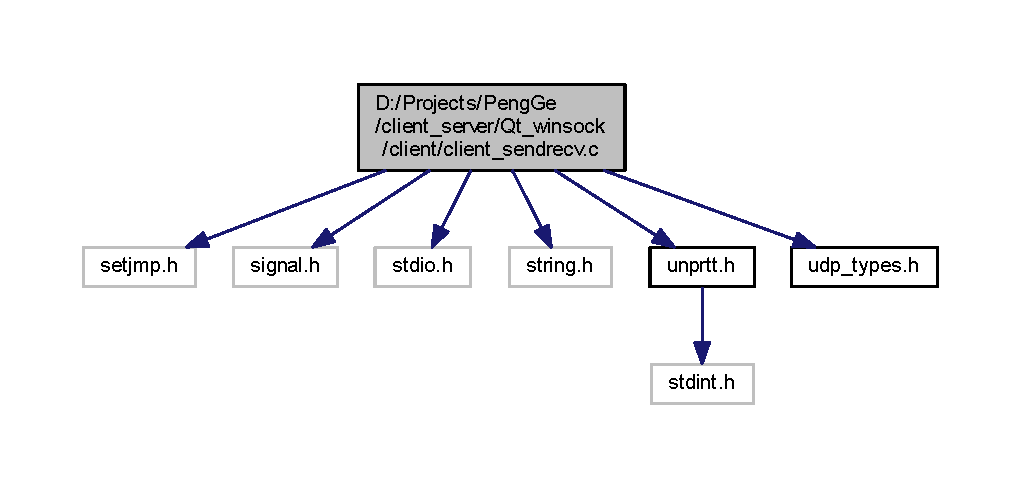
\includegraphics[width=350pt]{client__sendrecv_8c__incl}
\end{center}
\end{figure}
\subsection*{Macros}
\begin{DoxyCompactItemize}
\item 
\hypertarget{client__sendrecv_8c_af3b76ca76559f938a4f14abb1ad3e194}{}\#define {\bfseries bufptr}~void$\ast$\label{client__sendrecv_8c_af3b76ca76559f938a4f14abb1ad3e194}

\end{DoxyCompactItemize}
\subsection*{Functions}
\begin{DoxyCompactItemize}
\item 
\hypertarget{client__sendrecv_8c_a9aa91cdf73cc4fada27398ce0c7b5deb}{}ssize\+\_\+t {\bfseries client\+\_\+sendrecv} (S\+O\+C\+K\+E\+T fd, const void $\ast$outbuf, size\+\_\+t outbytes, void $\ast$inbuf, size\+\_\+t inbytes, const struct sockaddr $\ast$destaddr, int destlen)\label{client__sendrecv_8c_a9aa91cdf73cc4fada27398ce0c7b5deb}

\end{DoxyCompactItemize}


\subsection{Detailed Description}
\begin{DoxyAuthor}{Author}
cxl 
\end{DoxyAuthor}
\begin{DoxyVersion}{Version}
0.\+1 
\end{DoxyVersion}
\begin{DoxyDate}{Date}
2015-\/10-\/03 
\end{DoxyDate}

\hypertarget{client__udp_8c}{}\section{D\+:/project/\+Peng\+Ge/client\+\_\+server/src/client/client\+\_\+udp.c File Reference}
\label{client__udp_8c}\index{D\+:/project/\+Peng\+Ge/client\+\_\+server/src/client/client\+\_\+udp.\+c@{D\+:/project/\+Peng\+Ge/client\+\_\+server/src/client/client\+\_\+udp.\+c}}


This file prcess client udp message sendrecv. For now a lot config data is hard coded, reimplementation must be done when config parser complete.  


{\ttfamily \#include $<$sys/socket.\+h$>$}\\*
{\ttfamily \#include $<$netinet/in.\+h$>$}\\*
{\ttfamily \#include $<$pthread.\+h$>$}\\*
{\ttfamily \#include $<$unistd.\+h$>$}\\*
{\ttfamily \#include $<$assert.\+h$>$}\\*
{\ttfamily \#include $<$stdlib.\+h$>$}\\*
{\ttfamily \#include $<$stdio.\+h$>$}\\*
{\ttfamily \#include $<$stdint.\+h$>$}\\*
{\ttfamily \#include $<$string.\+h$>$}\\*
{\ttfamily \#include $<$semaphore.\+h$>$}\\*
{\ttfamily \#include \char`\"{}macros.\+h\char`\"{}}\\*
{\ttfamily \#include \char`\"{}bufarray.\+h\char`\"{}}\\*
{\ttfamily \#include \char`\"{}sock\+\_\+types.\+h\char`\"{}}\\*
{\ttfamily \#include \char`\"{}lightthread.\+h\char`\"{}}\\*
{\ttfamily \#include \char`\"{}utility\+\_\+wrap.\+h\char`\"{}}\\*
{\ttfamily \#include \char`\"{}msgpool.\+h\char`\"{}}\\*
{\ttfamily \#include \char`\"{}sock\+\_\+wrap.\+h\char`\"{}}\\*
{\ttfamily \#include \char`\"{}msgwrap.\+h\char`\"{}}\\*
{\ttfamily \#include \char`\"{}msgpool\+\_\+dispatch.\+h\char`\"{}}\\*
{\ttfamily \#include \char`\"{}client.\+h\char`\"{}}\\*
{\ttfamily \#include \char`\"{}client\+\_\+msgdispatch.\+h\char`\"{}}\\*
Include dependency graph for client\+\_\+udp.\+c\+:
\nopagebreak
\begin{figure}[H]
\begin{center}
\leavevmode
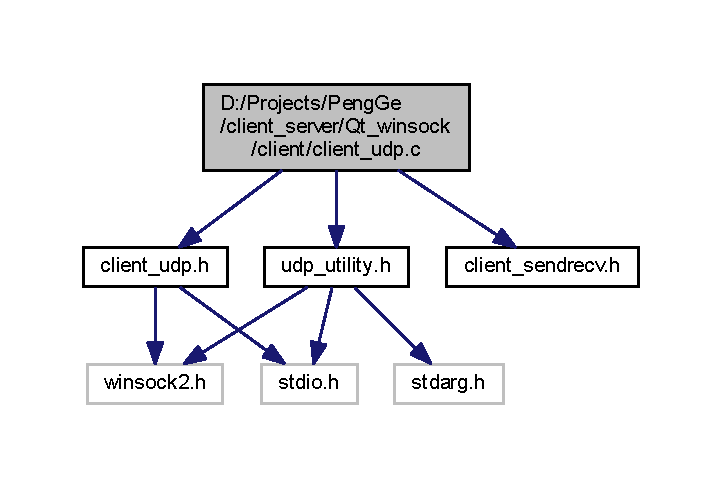
\includegraphics[width=350pt]{client__udp_8c__incl}
\end{center}
\end{figure}
\subsection*{Functions}
\begin{DoxyCompactItemize}
\item 
void \hyperlink{client__udp_8c_a8be5e8ba05fdac392536b4bb22d8914b}{csclient\+\_\+udp} (struct \hyperlink{structcsclient}{csclient} $\ast$cli, F\+I\+L\+E $\ast$fp, const struct sockaddr $\ast$servaddr, cssocklen\+\_\+t addrlen)
\begin{DoxyCompactList}\small\item\em csclient\+\_\+udp This function process udp communication with server. This function call csclient\+\_\+udp\+\_\+once in a loop. \end{DoxyCompactList}\item 
void \hyperlink{client__udp_8c_a571252c127c68c849fdf766d6cef63e2}{csclient\+\_\+udp\+\_\+once} (struct \hyperlink{structcsclient}{csclient} $\ast$cli, const struct sockaddr $\ast$servaddr, cssocklen\+\_\+t addrlen)
\begin{DoxyCompactList}\small\item\em csclient\+\_\+udp\+\_\+once This function process udp send\&recv one time. \end{DoxyCompactList}\end{DoxyCompactItemize}
\subsection*{Variables}
\begin{DoxyCompactItemize}
\item 
\hypertarget{client__udp_8c_a174a730c25e8784070b32a669e817448}{}const char $\ast$ {\bfseries g\+\_\+exit}\label{client__udp_8c_a174a730c25e8784070b32a669e817448}

\end{DoxyCompactItemize}


\subsection{Detailed Description}
This file prcess client udp message sendrecv. For now a lot config data is hard coded, reimplementation must be done when config parser complete. 

\begin{DoxyAuthor}{Author}
cxl, \href{mailto:shuanglongchen@yeah.net}{\tt shuanglongchen@yeah.\+net} 
\end{DoxyAuthor}
\begin{DoxyVersion}{Version}
0.\+1 
\end{DoxyVersion}
\begin{DoxyDate}{Date}
2015-\/11-\/07 
\end{DoxyDate}
\begin{DoxyParagraph}{last modified}
Sat 2015-\/11-\/07 15\+:57\+:32 (+0800) 
\end{DoxyParagraph}


\subsection{Function Documentation}
\hypertarget{client__udp_8c_a8be5e8ba05fdac392536b4bb22d8914b}{}\index{client\+\_\+udp.\+c@{client\+\_\+udp.\+c}!csclient\+\_\+udp@{csclient\+\_\+udp}}
\index{csclient\+\_\+udp@{csclient\+\_\+udp}!client\+\_\+udp.\+c@{client\+\_\+udp.\+c}}
\subsubsection[{csclient\+\_\+udp(struct csclient $\ast$cli, F\+I\+L\+E $\ast$fp, const struct sockaddr $\ast$servaddr, cssocklen\+\_\+t addrlen)}]{\setlength{\rightskip}{0pt plus 5cm}void csclient\+\_\+udp (
\begin{DoxyParamCaption}
\item[{struct {\bf csclient} $\ast$}]{cli, }
\item[{F\+I\+L\+E $\ast$}]{fp, }
\item[{const struct sockaddr $\ast$}]{servaddr, }
\item[{cssocklen\+\_\+t}]{addrlen}
\end{DoxyParamCaption}
)}\label{client__udp_8c_a8be5e8ba05fdac392536b4bb22d8914b}


csclient\+\_\+udp This function process udp communication with server. This function call csclient\+\_\+udp\+\_\+once in a loop. 


\begin{DoxyParams}{Parameters}
{\em cli} & \\
\hline
{\em fp} & is the F\+I\+L\+E pointer where input data comes from. \\
\hline
{\em servaddr} & \\
\hline
{\em addrlen} & \\
\hline
\end{DoxyParams}
\begin{DoxySeeAlso}{See also}
\hyperlink{client_8h_a571252c127c68c849fdf766d6cef63e2}{csclient\+\_\+udp\+\_\+once} 
\end{DoxySeeAlso}


Here is the call graph for this function\+:
\nopagebreak
\begin{figure}[H]
\begin{center}
\leavevmode
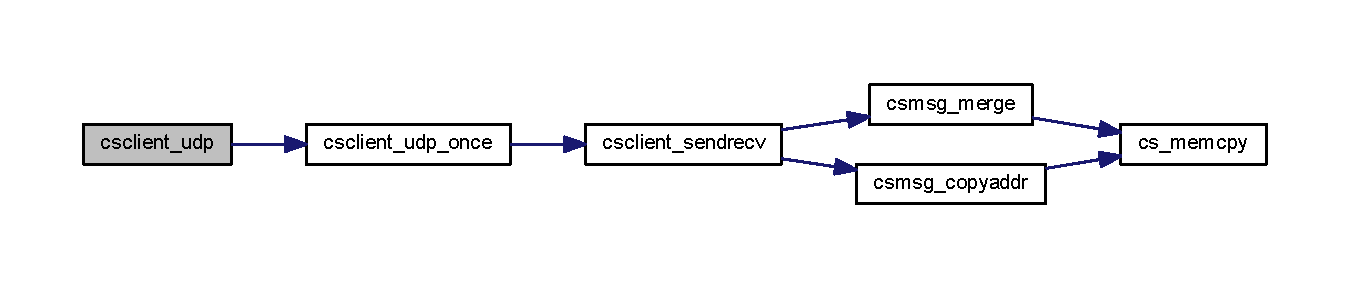
\includegraphics[width=350pt]{client__udp_8c_a8be5e8ba05fdac392536b4bb22d8914b_cgraph}
\end{center}
\end{figure}


\hypertarget{client__udp_8c_a571252c127c68c849fdf766d6cef63e2}{}\index{client\+\_\+udp.\+c@{client\+\_\+udp.\+c}!csclient\+\_\+udp\+\_\+once@{csclient\+\_\+udp\+\_\+once}}
\index{csclient\+\_\+udp\+\_\+once@{csclient\+\_\+udp\+\_\+once}!client\+\_\+udp.\+c@{client\+\_\+udp.\+c}}
\subsubsection[{csclient\+\_\+udp\+\_\+once(struct csclient $\ast$cli, const struct sockaddr $\ast$servaddr, cssocklen\+\_\+t addrlen)}]{\setlength{\rightskip}{0pt plus 5cm}void csclient\+\_\+udp\+\_\+once (
\begin{DoxyParamCaption}
\item[{struct {\bf csclient} $\ast$}]{cli, }
\item[{const struct sockaddr $\ast$}]{servaddr, }
\item[{cssocklen\+\_\+t}]{addrlen}
\end{DoxyParamCaption}
)}\label{client__udp_8c_a571252c127c68c849fdf766d6cef63e2}


csclient\+\_\+udp\+\_\+once This function process udp send\&recv one time. 


\begin{DoxyParams}{Parameters}
{\em cli} & cli has already been filled with data(end with \textquotesingle{}\textbackslash{}0\textquotesingle{}) to send. \\
\hline
{\em servaddr} & \\
\hline
{\em addrlen} & \\
\hline
\end{DoxyParams}


Here is the call graph for this function\+:
\nopagebreak
\begin{figure}[H]
\begin{center}
\leavevmode
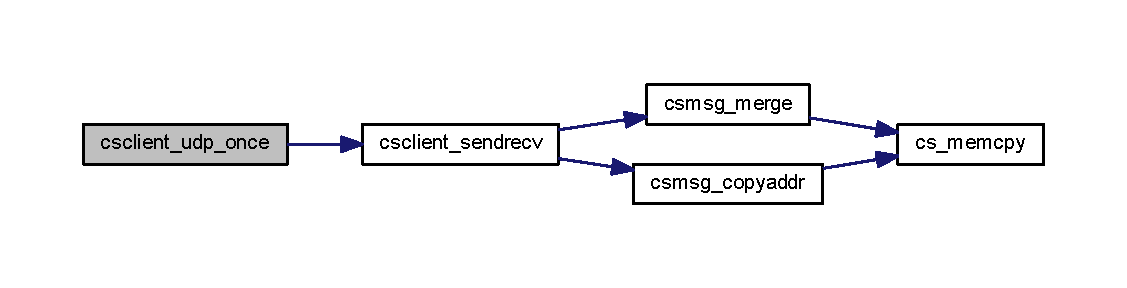
\includegraphics[width=350pt]{client__udp_8c_a571252c127c68c849fdf766d6cef63e2_cgraph}
\end{center}
\end{figure}




Here is the caller graph for this function\+:
\nopagebreak
\begin{figure}[H]
\begin{center}
\leavevmode
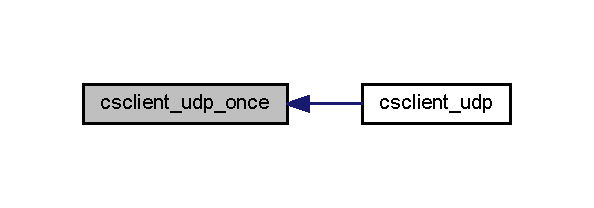
\includegraphics[width=285pt]{client__udp_8c_a571252c127c68c849fdf766d6cef63e2_icgraph}
\end{center}
\end{figure}



\hypertarget{client__udp_8h}{}\section{D\+:/\+Projects/\+Peng\+Ge/client\+\_\+server/\+Qt\+\_\+winsock/client/client\+\_\+udp.h File Reference}
\label{client__udp_8h}\index{D\+:/\+Projects/\+Peng\+Ge/client\+\_\+server/\+Qt\+\_\+winsock/client/client\+\_\+udp.\+h@{D\+:/\+Projects/\+Peng\+Ge/client\+\_\+server/\+Qt\+\_\+winsock/client/client\+\_\+udp.\+h}}


This file provide the interfaces of udp client.  


{\ttfamily \#include $<$stdio.\+h$>$}\\*
{\ttfamily \#include $<$winsock2.\+h$>$}\\*
Include dependency graph for client\+\_\+udp.\+h\+:
\nopagebreak
\begin{figure}[H]
\begin{center}
\leavevmode
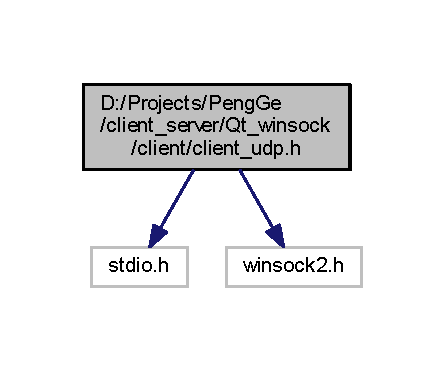
\includegraphics[width=214pt]{client__udp_8h__incl}
\end{center}
\end{figure}
This graph shows which files directly or indirectly include this file\+:
\nopagebreak
\begin{figure}[H]
\begin{center}
\leavevmode
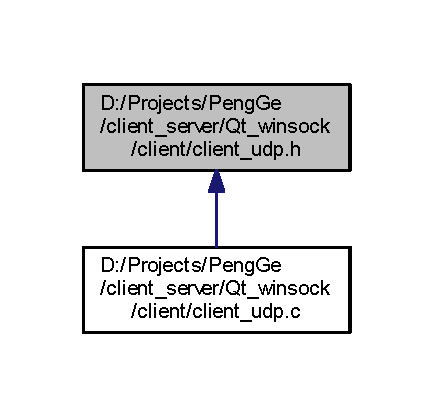
\includegraphics[width=208pt]{client__udp_8h__dep__incl}
\end{center}
\end{figure}
\subsection*{Classes}
\begin{DoxyCompactItemize}
\item 
struct \hyperlink{structclient__udp}{client\+\_\+udp}
\begin{DoxyCompactList}\small\item\em struct \hyperlink{structclient__udp}{client\+\_\+udp} contains necessary members and functions for client operations. This struct object must be initialized (by calling init\+\_\+client\+\_\+udp) before any operations applied to it. \end{DoxyCompactList}\end{DoxyCompactItemize}
\subsection*{Functions}
\begin{DoxyCompactItemize}
\item 
void \hyperlink{client__udp_8h_a3c6f803a771083053dac5e68b0f6d344}{check\+\_\+args} (int argc, char $\ast$argv\mbox{[}$\,$\mbox{]})
\begin{DoxyCompactList}\small\item\em check\+\_\+args checks whether the arguments are correct. If invalid paramters are passed, this function will give some prompts. \end{DoxyCompactList}\item 
void \hyperlink{client__udp_8h_a634ec1ea0f7527823a71d4c6a445425e}{init\+\_\+client\+\_\+udp} (struct \hyperlink{structclient__udp}{client\+\_\+udp} $\ast$cli\+\_\+udp)
\begin{DoxyCompactList}\small\item\em init\+\_\+client\+\_\+udp sets basic members and function pointers to the client object. \end{DoxyCompactList}\end{DoxyCompactItemize}


\subsection{Detailed Description}
This file provide the interfaces of udp client. 

\begin{DoxyAuthor}{Author}
cxl 
\end{DoxyAuthor}
\begin{DoxyVersion}{Version}
0.\+1 
\end{DoxyVersion}
\begin{DoxyDate}{Date}
2015-\/09-\/30 
\end{DoxyDate}


\subsection{Function Documentation}
\hypertarget{client__udp_8h_a3c6f803a771083053dac5e68b0f6d344}{}\index{client\+\_\+udp.\+h@{client\+\_\+udp.\+h}!check\+\_\+args@{check\+\_\+args}}
\index{check\+\_\+args@{check\+\_\+args}!client\+\_\+udp.\+h@{client\+\_\+udp.\+h}}
\subsubsection[{check\+\_\+args(int argc, char $\ast$argv[])}]{\setlength{\rightskip}{0pt plus 5cm}void check\+\_\+args (
\begin{DoxyParamCaption}
\item[{int}]{argc, }
\item[{char $\ast$}]{argv\mbox{[}$\,$\mbox{]}}
\end{DoxyParamCaption}
)}\label{client__udp_8h_a3c6f803a771083053dac5e68b0f6d344}


check\+\_\+args checks whether the arguments are correct. If invalid paramters are passed, this function will give some prompts. 


\begin{DoxyParams}{Parameters}
{\em argc} & \\
\hline
{\em argv\mbox{[}$\,$\mbox{]}} & \\
\hline
\end{DoxyParams}
\hypertarget{client__udp_8h_a634ec1ea0f7527823a71d4c6a445425e}{}\index{client\+\_\+udp.\+h@{client\+\_\+udp.\+h}!init\+\_\+client\+\_\+udp@{init\+\_\+client\+\_\+udp}}
\index{init\+\_\+client\+\_\+udp@{init\+\_\+client\+\_\+udp}!client\+\_\+udp.\+h@{client\+\_\+udp.\+h}}
\subsubsection[{init\+\_\+client\+\_\+udp(struct client\+\_\+udp $\ast$cli\+\_\+udp)}]{\setlength{\rightskip}{0pt plus 5cm}void init\+\_\+client\+\_\+udp (
\begin{DoxyParamCaption}
\item[{struct {\bf client\+\_\+udp} $\ast$}]{cli\+\_\+udp}
\end{DoxyParamCaption}
)}\label{client__udp_8h_a634ec1ea0f7527823a71d4c6a445425e}


init\+\_\+client\+\_\+udp sets basic members and function pointers to the client object. 


\begin{DoxyParams}{Parameters}
{\em cli\+\_\+udp} & \\
\hline
\end{DoxyParams}
\begin{DoxyNote}{Note}
This function must be called immediately after W\+S\+A\+Startup being called. 
\end{DoxyNote}

\hypertarget{unprtt_8h}{}\section{D\+:/\+Projects/\+Peng\+Ge/client\+\_\+server/\+Qt\+\_\+winsock/client/unprtt.h File Reference}
\label{unprtt_8h}\index{D\+:/\+Projects/\+Peng\+Ge/client\+\_\+server/\+Qt\+\_\+winsock/client/unprtt.\+h@{D\+:/\+Projects/\+Peng\+Ge/client\+\_\+server/\+Qt\+\_\+winsock/client/unprtt.\+h}}


This file comes from \textquotesingle{}U\+N\+I\+X Network Programming\textquotesingle{} source code.  


{\ttfamily \#include $<$stdint.\+h$>$}\\*
Include dependency graph for unprtt.\+h\+:
\nopagebreak
\begin{figure}[H]
\begin{center}
\leavevmode
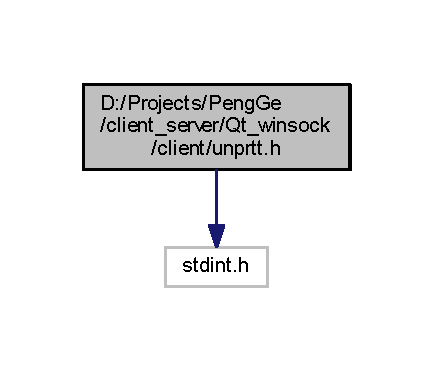
\includegraphics[width=208pt]{unprtt_8h__incl}
\end{center}
\end{figure}
This graph shows which files directly or indirectly include this file\+:
\nopagebreak
\begin{figure}[H]
\begin{center}
\leavevmode
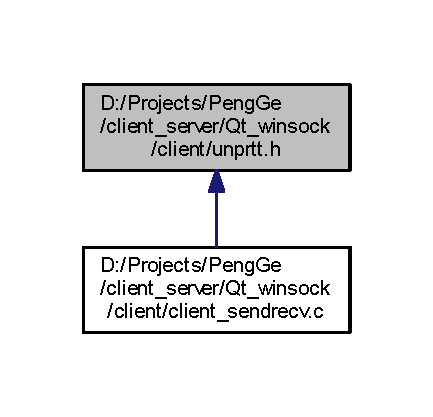
\includegraphics[width=208pt]{unprtt_8h__dep__incl}
\end{center}
\end{figure}
\subsection*{Classes}
\begin{DoxyCompactItemize}
\item 
struct \hyperlink{structrtt__info}{rtt\+\_\+info}
\end{DoxyCompactItemize}
\subsection*{Macros}
\begin{DoxyCompactItemize}
\item 
\hypertarget{unprtt_8h_a003daf6b4ebfd9ade32edfeb677d3f74}{}\#define {\bfseries R\+T\+T\+\_\+\+R\+X\+T\+M\+I\+N}~2	/$\ast$ min retransmit timeout value, in seconds $\ast$/\label{unprtt_8h_a003daf6b4ebfd9ade32edfeb677d3f74}

\item 
\hypertarget{unprtt_8h_afd5140f29c60ceb157befe7691a097ed}{}\#define {\bfseries R\+T\+T\+\_\+\+R\+X\+T\+M\+A\+X}~60	/$\ast$ max retransmit timeout value, in seconds $\ast$/\label{unprtt_8h_afd5140f29c60ceb157befe7691a097ed}

\item 
\hypertarget{unprtt_8h_a672e9e317a9d4cb8c9f62b121757e81d}{}\#define {\bfseries R\+T\+T\+\_\+\+M\+A\+X\+N\+R\+E\+X\+M\+T}~3	/$\ast$ max \# times to retransmit $\ast$/\label{unprtt_8h_a672e9e317a9d4cb8c9f62b121757e81d}

\end{DoxyCompactItemize}
\subsection*{Functions}
\begin{DoxyCompactItemize}
\item 
\hypertarget{unprtt_8h_a3741468280b31358eb140ec9ad8b7748}{}void {\bfseries rtt\+\_\+debug} (struct \hyperlink{structrtt__info}{rtt\+\_\+info} $\ast$)\label{unprtt_8h_a3741468280b31358eb140ec9ad8b7748}

\item 
\hypertarget{unprtt_8h_a0287d720e1beefe26654495345dcfea0}{}void {\bfseries rtt\+\_\+init} (struct \hyperlink{structrtt__info}{rtt\+\_\+info} $\ast$)\label{unprtt_8h_a0287d720e1beefe26654495345dcfea0}

\item 
\hypertarget{unprtt_8h_ae4a0c480601fb4e591b734050d18739b}{}void {\bfseries rtt\+\_\+newpack} (struct \hyperlink{structrtt__info}{rtt\+\_\+info} $\ast$)\label{unprtt_8h_ae4a0c480601fb4e591b734050d18739b}

\item 
\hypertarget{unprtt_8h_ad78cae7d6369311b9164501a3f8b948a}{}int {\bfseries rtt\+\_\+start} (struct \hyperlink{structrtt__info}{rtt\+\_\+info} $\ast$)\label{unprtt_8h_ad78cae7d6369311b9164501a3f8b948a}

\item 
\hypertarget{unprtt_8h_a45423ff010c73c75ecc3d4bf55558682}{}void {\bfseries rtt\+\_\+stop} (struct \hyperlink{structrtt__info}{rtt\+\_\+info} $\ast$, uint32\+\_\+t)\label{unprtt_8h_a45423ff010c73c75ecc3d4bf55558682}

\item 
\hypertarget{unprtt_8h_a4e3fbd4c76174a02fc6992f333a90054}{}int {\bfseries rtt\+\_\+timeout} (struct \hyperlink{structrtt__info}{rtt\+\_\+info} $\ast$)\label{unprtt_8h_a4e3fbd4c76174a02fc6992f333a90054}

\item 
\hypertarget{unprtt_8h_ae60a79e3fdd3a8c76e2f336d9984498f}{}uint32\+\_\+t {\bfseries rtt\+\_\+ts} (struct \hyperlink{structrtt__info}{rtt\+\_\+info} $\ast$)\label{unprtt_8h_ae60a79e3fdd3a8c76e2f336d9984498f}

\end{DoxyCompactItemize}
\subsection*{Variables}
\begin{DoxyCompactItemize}
\item 
\hypertarget{unprtt_8h_a7c7ad1b4e2182b95b294b91a3b5e2ca2}{}int {\bfseries rtt\+\_\+d\+\_\+flag}\label{unprtt_8h_a7c7ad1b4e2182b95b294b91a3b5e2ca2}

\end{DoxyCompactItemize}


\subsection{Detailed Description}
This file comes from \textquotesingle{}U\+N\+I\+X Network Programming\textquotesingle{} source code. 

\begin{DoxyAuthor}{Author}
cxl 
\end{DoxyAuthor}
\begin{DoxyVersion}{Version}
0.\+1 
\end{DoxyVersion}
\begin{DoxyDate}{Date}
2015-\/10-\/09 
\end{DoxyDate}

\hypertarget{udp__types_8h}{}\section{D\+:/\+Projects/\+Peng\+Ge/client\+\_\+server/\+Qt\+\_\+winsock/common/udp\+\_\+types.h File Reference}
\label{udp__types_8h}\index{D\+:/\+Projects/\+Peng\+Ge/client\+\_\+server/\+Qt\+\_\+winsock/common/udp\+\_\+types.\+h@{D\+:/\+Projects/\+Peng\+Ge/client\+\_\+server/\+Qt\+\_\+winsock/common/udp\+\_\+types.\+h}}
This graph shows which files directly or indirectly include this file\+:
\nopagebreak
\begin{figure}[H]
\begin{center}
\leavevmode
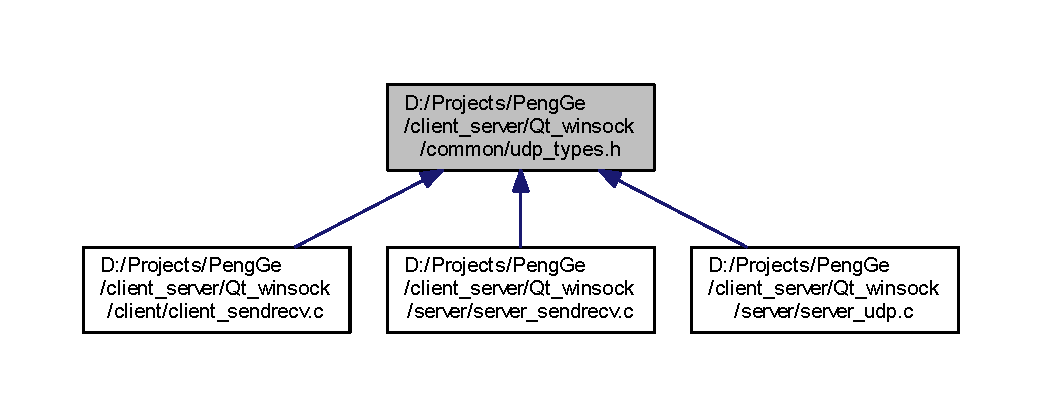
\includegraphics[width=350pt]{udp__types_8h__dep__incl}
\end{center}
\end{figure}
\subsection*{Classes}
\begin{DoxyCompactItemize}
\item 
struct \hyperlink{structhdr}{hdr}
\end{DoxyCompactItemize}


\subsection{Detailed Description}
\begin{DoxyAuthor}{Author}
cxl 
\end{DoxyAuthor}
\begin{DoxyVersion}{Version}
0.\+1 
\end{DoxyVersion}
\begin{DoxyDate}{Date}
2015-\/10-\/10 
\end{DoxyDate}

\hypertarget{udp__utility_8c}{}\section{D\+:/\+Projects/\+Peng\+Ge/client\+\_\+server/\+Qt\+\_\+winsock/common/udp\+\_\+utility.c File Reference}
\label{udp__utility_8c}\index{D\+:/\+Projects/\+Peng\+Ge/client\+\_\+server/\+Qt\+\_\+winsock/common/udp\+\_\+utility.\+c@{D\+:/\+Projects/\+Peng\+Ge/client\+\_\+server/\+Qt\+\_\+winsock/common/udp\+\_\+utility.\+c}}
{\ttfamily \#include $<$stdio.\+h$>$}\\*
{\ttfamily \#include $<$stdlib.\+h$>$}\\*
{\ttfamily \#include \char`\"{}udp\+\_\+utility.\+h\char`\"{}}\\*
Include dependency graph for udp\+\_\+utility.\+c\+:
\nopagebreak
\begin{figure}[H]
\begin{center}
\leavevmode
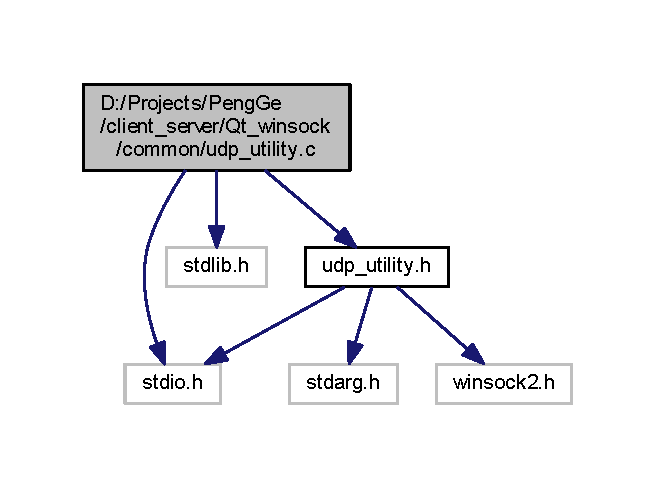
\includegraphics[width=315pt]{udp__utility_8c__incl}
\end{center}
\end{figure}
\subsection*{Functions}
\begin{DoxyCompactItemize}
\item 
void \hyperlink{udp__utility_8c_aded12ee524c5f45b7d4c0392e14c6d9b}{U\+\_\+errexit} (const char $\ast$format,...)
\begin{DoxyCompactList}\small\item\em U\+\_\+errexit Print error information and exit(1). \end{DoxyCompactList}\item 
void \hyperlink{udp__utility_8c_ac4419ec449365c1ef66d1386686f55b3}{U\+\_\+errexit\+\_\+value} (int exit\+\_\+value, const char $\ast$format,...)
\begin{DoxyCompactList}\small\item\em U\+\_\+errexit\+\_\+value Print error information and exit(exit\+\_\+value). \end{DoxyCompactList}\item 
void \hyperlink{udp__utility_8c_adb05a762c0dc472cf20efee8d3a6433f}{U\+\_\+init\+\_\+winsock2} (W\+S\+A\+D\+A\+T\+A $\ast$wsadata)
\begin{DoxyCompactList}\small\item\em U\+\_\+init\+\_\+winsock2 Wrapped function of W\+S\+A\+Startup with error checking. \end{DoxyCompactList}\item 
\hypertarget{udp__utility_8c_ad4c0a2157c32294878ca530018ff5175}{}void \hyperlink{udp__utility_8c_ad4c0a2157c32294878ca530018ff5175}{U\+\_\+cleanup\+\_\+winsock2} ()\label{udp__utility_8c_ad4c0a2157c32294878ca530018ff5175}

\begin{DoxyCompactList}\small\item\em U\+\_\+cleanup\+\_\+winsock2 Wrapped function of W\+S\+A\+Cleanup with error checking When your application is finished handling the connections, call W\+S\+A\+Cleanup. \end{DoxyCompactList}\item 
void \hyperlink{udp__utility_8c_aeb6a91ab17e7927f3a4c046e637d66af}{U\+\_\+close\+\_\+socket} (S\+O\+C\+K\+E\+T sockfd)
\begin{DoxyCompactList}\small\item\em U\+\_\+close\+\_\+socket closesocket() wrapper with error checking. \end{DoxyCompactList}\item 
\hypertarget{udp__utility_8c_a73f1cfc1470e06a6cb8eafb0b65a8c89}{}int {\bfseries U\+\_\+printf\+\_\+sockinfo} (S\+O\+C\+K\+E\+T sockfd, char $\ast$msgheader)\label{udp__utility_8c_a73f1cfc1470e06a6cb8eafb0b65a8c89}

\end{DoxyCompactItemize}
\subsection*{Variables}
\begin{DoxyCompactItemize}
\item 
\hypertarget{udp__utility_8c_a4520db064bea79e42630a63a529a450c}{}const char $\ast$ {\bfseries g\+\_\+loginmsg\+\_\+header} = \char`\"{}login\+: \char`\"{}\label{udp__utility_8c_a4520db064bea79e42630a63a529a450c}

\item 
\hypertarget{udp__utility_8c_a60cacc9239d0662a686899339cf5b127}{}const char $\ast$ {\bfseries g\+\_\+loginmsg\+\_\+\+S\+U\+C\+C\+E\+S\+S} = \char`\"{}login\+\_\+success\char`\"{}\label{udp__utility_8c_a60cacc9239d0662a686899339cf5b127}

\item 
\hypertarget{udp__utility_8c_ab241e51fd6b4014566bd16db0e23de58}{}const char $\ast$ {\bfseries g\+\_\+loginmsg\+\_\+\+F\+A\+I\+L} = \char`\"{}login\+\_\+fail\char`\"{}\label{udp__utility_8c_ab241e51fd6b4014566bd16db0e23de58}

\item 
\hypertarget{udp__utility_8c_a533bdde78cc9c28ca1a7c9418177f6a7}{}const char {\bfseries g\+\_\+login\+\_\+delimiter} = \textquotesingle{} \textquotesingle{}\label{udp__utility_8c_a533bdde78cc9c28ca1a7c9418177f6a7}

\end{DoxyCompactItemize}


\subsection{Detailed Description}
\begin{DoxyAuthor}{Author}
cxl 
\end{DoxyAuthor}
\begin{DoxyVersion}{Version}
0.\+1 
\end{DoxyVersion}
\begin{DoxyDate}{Date}
2015-\/09-\/20 
\end{DoxyDate}


\subsection{Function Documentation}
\hypertarget{udp__utility_8c_aeb6a91ab17e7927f3a4c046e637d66af}{}\index{udp\+\_\+utility.\+c@{udp\+\_\+utility.\+c}!U\+\_\+close\+\_\+socket@{U\+\_\+close\+\_\+socket}}
\index{U\+\_\+close\+\_\+socket@{U\+\_\+close\+\_\+socket}!udp\+\_\+utility.\+c@{udp\+\_\+utility.\+c}}
\subsubsection[{U\+\_\+close\+\_\+socket(\+S\+O\+C\+K\+E\+T sockfd)}]{\setlength{\rightskip}{0pt plus 5cm}void U\+\_\+close\+\_\+socket (
\begin{DoxyParamCaption}
\item[{S\+O\+C\+K\+E\+T}]{sockfd}
\end{DoxyParamCaption}
)}\label{udp__utility_8c_aeb6a91ab17e7927f3a4c046e637d66af}


U\+\_\+close\+\_\+socket closesocket() wrapper with error checking. 


\begin{DoxyParams}{Parameters}
{\em sockfd} & socket to close \\
\hline
\end{DoxyParams}
\hypertarget{udp__utility_8c_aded12ee524c5f45b7d4c0392e14c6d9b}{}\index{udp\+\_\+utility.\+c@{udp\+\_\+utility.\+c}!U\+\_\+errexit@{U\+\_\+errexit}}
\index{U\+\_\+errexit@{U\+\_\+errexit}!udp\+\_\+utility.\+c@{udp\+\_\+utility.\+c}}
\subsubsection[{U\+\_\+errexit(const char $\ast$format,...)}]{\setlength{\rightskip}{0pt plus 5cm}void U\+\_\+errexit (
\begin{DoxyParamCaption}
\item[{const char $\ast$}]{format, }
\item[{}]{...}
\end{DoxyParamCaption}
)}\label{udp__utility_8c_aded12ee524c5f45b7d4c0392e14c6d9b}


U\+\_\+errexit Print error information and exit(1). 


\begin{DoxyParams}{Parameters}
{\em format} & \\
\hline
{\em ...} & \\
\hline
\end{DoxyParams}
\hypertarget{udp__utility_8c_ac4419ec449365c1ef66d1386686f55b3}{}\index{udp\+\_\+utility.\+c@{udp\+\_\+utility.\+c}!U\+\_\+errexit\+\_\+value@{U\+\_\+errexit\+\_\+value}}
\index{U\+\_\+errexit\+\_\+value@{U\+\_\+errexit\+\_\+value}!udp\+\_\+utility.\+c@{udp\+\_\+utility.\+c}}
\subsubsection[{U\+\_\+errexit\+\_\+value(int exit\+\_\+value, const char $\ast$format,...)}]{\setlength{\rightskip}{0pt plus 5cm}void U\+\_\+errexit\+\_\+value (
\begin{DoxyParamCaption}
\item[{int}]{exit\+\_\+value, }
\item[{const char $\ast$}]{format, }
\item[{}]{...}
\end{DoxyParamCaption}
)}\label{udp__utility_8c_ac4419ec449365c1ef66d1386686f55b3}


U\+\_\+errexit\+\_\+value Print error information and exit(exit\+\_\+value). 


\begin{DoxyParams}{Parameters}
{\em exit\+\_\+value} & value for exit() \\
\hline
{\em format} & \\
\hline
{\em ...} & \\
\hline
\end{DoxyParams}
\hypertarget{udp__utility_8c_adb05a762c0dc472cf20efee8d3a6433f}{}\index{udp\+\_\+utility.\+c@{udp\+\_\+utility.\+c}!U\+\_\+init\+\_\+winsock2@{U\+\_\+init\+\_\+winsock2}}
\index{U\+\_\+init\+\_\+winsock2@{U\+\_\+init\+\_\+winsock2}!udp\+\_\+utility.\+c@{udp\+\_\+utility.\+c}}
\subsubsection[{U\+\_\+init\+\_\+winsock2(\+W\+S\+A\+D\+A\+T\+A $\ast$wsadata)}]{\setlength{\rightskip}{0pt plus 5cm}void U\+\_\+init\+\_\+winsock2 (
\begin{DoxyParamCaption}
\item[{W\+S\+A\+D\+A\+T\+A $\ast$}]{wsadata}
\end{DoxyParamCaption}
)}\label{udp__utility_8c_adb05a762c0dc472cf20efee8d3a6433f}


U\+\_\+init\+\_\+winsock2 Wrapped function of W\+S\+A\+Startup with error checking. 


\begin{DoxyParams}{Parameters}
{\em wsadata} & \\
\hline
\end{DoxyParams}

\hypertarget{udp__utility_8h}{}\section{D\+:/\+Projects/\+Peng\+Ge/client\+\_\+server/\+Qt\+\_\+winsock/common/udp\+\_\+utility.h File Reference}
\label{udp__utility_8h}\index{D\+:/\+Projects/\+Peng\+Ge/client\+\_\+server/\+Qt\+\_\+winsock/common/udp\+\_\+utility.\+h@{D\+:/\+Projects/\+Peng\+Ge/client\+\_\+server/\+Qt\+\_\+winsock/common/udp\+\_\+utility.\+h}}


Utility functions. The prefix \char`\"{}\+U\+\_\+\char`\"{} stands for utility.  


{\ttfamily \#include $<$stdarg.\+h$>$}\\*
{\ttfamily \#include $<$winsock2.\+h$>$}\\*
{\ttfamily \#include $<$stdio.\+h$>$}\\*
Include dependency graph for udp\+\_\+utility.\+h\+:
\nopagebreak
\begin{figure}[H]
\begin{center}
\leavevmode
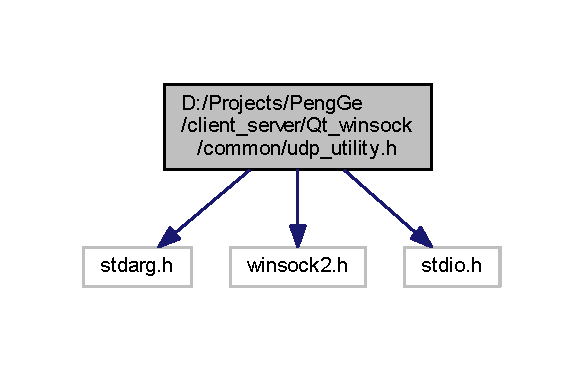
\includegraphics[width=280pt]{udp__utility_8h__incl}
\end{center}
\end{figure}
This graph shows which files directly or indirectly include this file\+:
\nopagebreak
\begin{figure}[H]
\begin{center}
\leavevmode
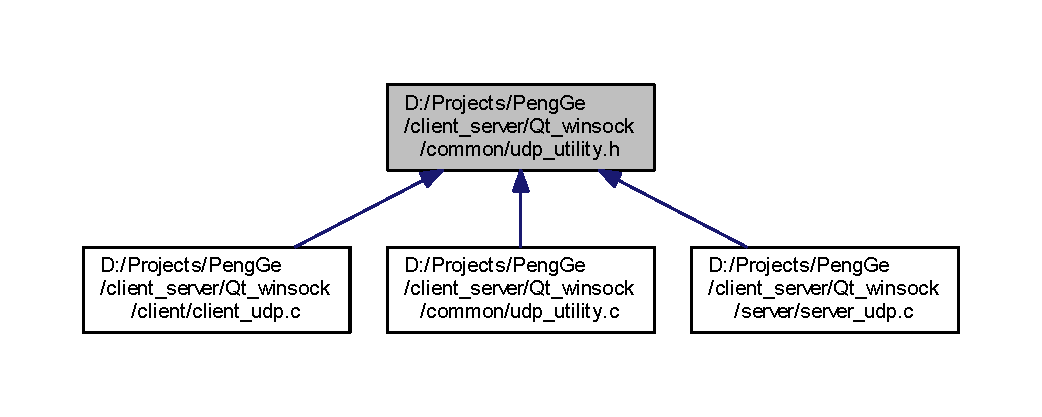
\includegraphics[width=350pt]{udp__utility_8h__dep__incl}
\end{center}
\end{figure}
\subsection*{Functions}
\begin{DoxyCompactItemize}
\item 
void \hyperlink{udp__utility_8h_aded12ee524c5f45b7d4c0392e14c6d9b}{U\+\_\+errexit} (const char $\ast$format,...)
\begin{DoxyCompactList}\small\item\em U\+\_\+errexit Print error information and exit(1). \end{DoxyCompactList}\item 
void \hyperlink{udp__utility_8h_ac4419ec449365c1ef66d1386686f55b3}{U\+\_\+errexit\+\_\+value} (int exit\+\_\+value, const char $\ast$format,...)
\begin{DoxyCompactList}\small\item\em U\+\_\+errexit\+\_\+value Print error information and exit(exit\+\_\+value). \end{DoxyCompactList}\item 
void \hyperlink{udp__utility_8h_adb05a762c0dc472cf20efee8d3a6433f}{U\+\_\+init\+\_\+winsock2} (W\+S\+A\+D\+A\+T\+A $\ast$wsadata)
\begin{DoxyCompactList}\small\item\em U\+\_\+init\+\_\+winsock2 Wrapped function of W\+S\+A\+Startup with error checking. \end{DoxyCompactList}\item 
void \hyperlink{udp__utility_8h_aeb6a91ab17e7927f3a4c046e637d66af}{U\+\_\+close\+\_\+socket} (S\+O\+C\+K\+E\+T sockfd)
\begin{DoxyCompactList}\small\item\em U\+\_\+close\+\_\+socket closesocket() wrapper with error checking. \end{DoxyCompactList}\item 
\hypertarget{udp__utility_8h_a40fe718aed79325649f9488a38918e14}{}void \hyperlink{udp__utility_8h_a40fe718aed79325649f9488a38918e14}{U\+\_\+cleanup\+\_\+winsock2} (void)\label{udp__utility_8h_a40fe718aed79325649f9488a38918e14}

\begin{DoxyCompactList}\small\item\em U\+\_\+cleanup\+\_\+winsock2 Wrapped function of W\+S\+A\+Cleanup with error checking When your application is finished handling the connections, call W\+S\+A\+Cleanup. \end{DoxyCompactList}\item 
\hypertarget{udp__utility_8h_a73f1cfc1470e06a6cb8eafb0b65a8c89}{}int {\bfseries U\+\_\+printf\+\_\+sockinfo} (S\+O\+C\+K\+E\+T sockfd, char $\ast$msgheader)\label{udp__utility_8h_a73f1cfc1470e06a6cb8eafb0b65a8c89}

\end{DoxyCompactItemize}


\subsection{Detailed Description}
Utility functions. The prefix \char`\"{}\+U\+\_\+\char`\"{} stands for utility. 

\begin{DoxyAuthor}{Author}
cxl 
\end{DoxyAuthor}
\begin{DoxyVersion}{Version}
0.\+1 
\end{DoxyVersion}
\begin{DoxyDate}{Date}
2015-\/09-\/20 
\end{DoxyDate}


\subsection{Function Documentation}
\hypertarget{udp__utility_8h_aeb6a91ab17e7927f3a4c046e637d66af}{}\index{udp\+\_\+utility.\+h@{udp\+\_\+utility.\+h}!U\+\_\+close\+\_\+socket@{U\+\_\+close\+\_\+socket}}
\index{U\+\_\+close\+\_\+socket@{U\+\_\+close\+\_\+socket}!udp\+\_\+utility.\+h@{udp\+\_\+utility.\+h}}
\subsubsection[{U\+\_\+close\+\_\+socket(\+S\+O\+C\+K\+E\+T sockfd)}]{\setlength{\rightskip}{0pt plus 5cm}void U\+\_\+close\+\_\+socket (
\begin{DoxyParamCaption}
\item[{S\+O\+C\+K\+E\+T}]{sockfd}
\end{DoxyParamCaption}
)}\label{udp__utility_8h_aeb6a91ab17e7927f3a4c046e637d66af}


U\+\_\+close\+\_\+socket closesocket() wrapper with error checking. 


\begin{DoxyParams}{Parameters}
{\em sockfd} & socket to close \\
\hline
\end{DoxyParams}
\hypertarget{udp__utility_8h_aded12ee524c5f45b7d4c0392e14c6d9b}{}\index{udp\+\_\+utility.\+h@{udp\+\_\+utility.\+h}!U\+\_\+errexit@{U\+\_\+errexit}}
\index{U\+\_\+errexit@{U\+\_\+errexit}!udp\+\_\+utility.\+h@{udp\+\_\+utility.\+h}}
\subsubsection[{U\+\_\+errexit(const char $\ast$format,...)}]{\setlength{\rightskip}{0pt plus 5cm}void U\+\_\+errexit (
\begin{DoxyParamCaption}
\item[{const char $\ast$}]{format, }
\item[{}]{...}
\end{DoxyParamCaption}
)}\label{udp__utility_8h_aded12ee524c5f45b7d4c0392e14c6d9b}


U\+\_\+errexit Print error information and exit(1). 


\begin{DoxyParams}{Parameters}
{\em format} & \\
\hline
{\em ...} & \\
\hline
\end{DoxyParams}
\hypertarget{udp__utility_8h_ac4419ec449365c1ef66d1386686f55b3}{}\index{udp\+\_\+utility.\+h@{udp\+\_\+utility.\+h}!U\+\_\+errexit\+\_\+value@{U\+\_\+errexit\+\_\+value}}
\index{U\+\_\+errexit\+\_\+value@{U\+\_\+errexit\+\_\+value}!udp\+\_\+utility.\+h@{udp\+\_\+utility.\+h}}
\subsubsection[{U\+\_\+errexit\+\_\+value(int exit\+\_\+value, const char $\ast$format,...)}]{\setlength{\rightskip}{0pt plus 5cm}void U\+\_\+errexit\+\_\+value (
\begin{DoxyParamCaption}
\item[{int}]{exit\+\_\+value, }
\item[{const char $\ast$}]{format, }
\item[{}]{...}
\end{DoxyParamCaption}
)}\label{udp__utility_8h_ac4419ec449365c1ef66d1386686f55b3}


U\+\_\+errexit\+\_\+value Print error information and exit(exit\+\_\+value). 


\begin{DoxyParams}{Parameters}
{\em exit\+\_\+value} & value for exit() \\
\hline
{\em format} & \\
\hline
{\em ...} & \\
\hline
\end{DoxyParams}
\hypertarget{udp__utility_8h_adb05a762c0dc472cf20efee8d3a6433f}{}\index{udp\+\_\+utility.\+h@{udp\+\_\+utility.\+h}!U\+\_\+init\+\_\+winsock2@{U\+\_\+init\+\_\+winsock2}}
\index{U\+\_\+init\+\_\+winsock2@{U\+\_\+init\+\_\+winsock2}!udp\+\_\+utility.\+h@{udp\+\_\+utility.\+h}}
\subsubsection[{U\+\_\+init\+\_\+winsock2(\+W\+S\+A\+D\+A\+T\+A $\ast$wsadata)}]{\setlength{\rightskip}{0pt plus 5cm}void U\+\_\+init\+\_\+winsock2 (
\begin{DoxyParamCaption}
\item[{W\+S\+A\+D\+A\+T\+A $\ast$}]{wsadata}
\end{DoxyParamCaption}
)}\label{udp__utility_8h_adb05a762c0dc472cf20efee8d3a6433f}


U\+\_\+init\+\_\+winsock2 Wrapped function of W\+S\+A\+Startup with error checking. 


\begin{DoxyParams}{Parameters}
{\em wsadata} & \\
\hline
\end{DoxyParams}

\hypertarget{server__sendrecv_8c}{}\section{D\+:/\+Projects/\+Peng\+Ge/client\+\_\+server/\+Qt\+\_\+winsock/server/server\+\_\+sendrecv.c File Reference}
\label{server__sendrecv_8c}\index{D\+:/\+Projects/\+Peng\+Ge/client\+\_\+server/\+Qt\+\_\+winsock/server/server\+\_\+sendrecv.\+c@{D\+:/\+Projects/\+Peng\+Ge/client\+\_\+server/\+Qt\+\_\+winsock/server/server\+\_\+sendrecv.\+c}}
{\ttfamily \#include $<$string.\+h$>$}\\*
{\ttfamily \#include $<$stdio.\+h$>$}\\*
{\ttfamily \#include $<$stdint.\+h$>$}\\*
{\ttfamily \#include \char`\"{}udp\+\_\+types.\+h\char`\"{}}\\*
Include dependency graph for server\+\_\+sendrecv.\+c\+:
\nopagebreak
\begin{figure}[H]
\begin{center}
\leavevmode
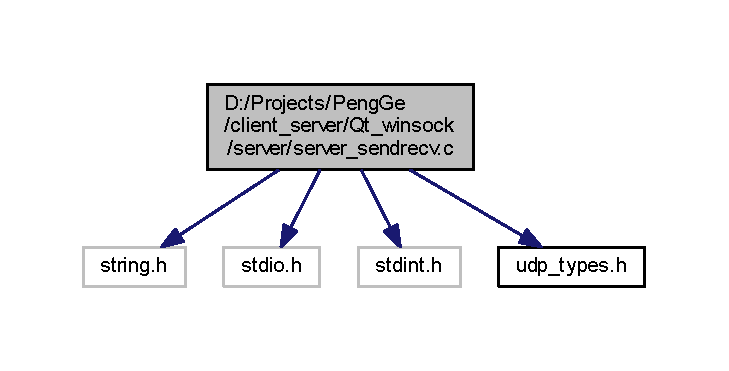
\includegraphics[width=350pt]{server__sendrecv_8c__incl}
\end{center}
\end{figure}
\subsection*{Macros}
\begin{DoxyCompactItemize}
\item 
\hypertarget{server__sendrecv_8c_af3b76ca76559f938a4f14abb1ad3e194}{}\#define {\bfseries bufptr}~void$\ast$\label{server__sendrecv_8c_af3b76ca76559f938a4f14abb1ad3e194}

\item 
\hypertarget{server__sendrecv_8c_af3b76ca76559f938a4f14abb1ad3e194}{}\#define {\bfseries bufptr}~void$\ast$\label{server__sendrecv_8c_af3b76ca76559f938a4f14abb1ad3e194}

\end{DoxyCompactItemize}
\subsection*{Functions}
\begin{DoxyCompactItemize}
\item 
ssize\+\_\+t \hyperlink{server__sendrecv_8c_abbf550e967157f1f7a9435ecf62787c4}{server\+\_\+recv} (S\+O\+C\+K\+E\+T fd, void $\ast$inbuf, size\+\_\+t inbytes, struct \hyperlink{structhdr}{hdr} $\ast$hdrdata, struct sockaddr $\ast$cli\+\_\+addr, int $\ast$cli\+\_\+addrlen)
\item 
\hypertarget{server__sendrecv_8c_aa859f524235db38e2161366b5ab660c6}{}void {\bfseries server\+\_\+send} (S\+O\+C\+K\+E\+T fd, const void $\ast$outbuf, size\+\_\+t outbytes, const struct \hyperlink{structhdr}{hdr} $\ast$hdrdata, const struct sockaddr $\ast$cli\+\_\+addr, int cli\+\_\+addrlen)\label{server__sendrecv_8c_aa859f524235db38e2161366b5ab660c6}

\end{DoxyCompactItemize}


\subsection{Detailed Description}
\begin{DoxyAuthor}{Author}
cxl 
\end{DoxyAuthor}
\begin{DoxyVersion}{Version}
0.\+1 
\end{DoxyVersion}
\begin{DoxyDate}{Date}
2015-\/10-\/10 
\end{DoxyDate}


\subsection{Function Documentation}
\hypertarget{server__sendrecv_8c_abbf550e967157f1f7a9435ecf62787c4}{}\index{server\+\_\+sendrecv.\+c@{server\+\_\+sendrecv.\+c}!server\+\_\+recv@{server\+\_\+recv}}
\index{server\+\_\+recv@{server\+\_\+recv}!server\+\_\+sendrecv.\+c@{server\+\_\+sendrecv.\+c}}
\subsubsection[{server\+\_\+recv(\+S\+O\+C\+K\+E\+T fd, void $\ast$inbuf, size\+\_\+t inbytes, struct hdr $\ast$hdrdata, struct sockaddr $\ast$cli\+\_\+addr, int $\ast$cli\+\_\+addrlen)}]{\setlength{\rightskip}{0pt plus 5cm}ssize\+\_\+t server\+\_\+recv (
\begin{DoxyParamCaption}
\item[{S\+O\+C\+K\+E\+T}]{fd, }
\item[{void $\ast$}]{inbuf, }
\item[{size\+\_\+t}]{inbytes, }
\item[{struct {\bf hdr} $\ast$}]{hdrdata, }
\item[{struct sockaddr $\ast$}]{cli\+\_\+addr, }
\item[{int $\ast$}]{cli\+\_\+addrlen}
\end{DoxyParamCaption}
)}\label{server__sendrecv_8c_abbf550e967157f1f7a9435ecf62787c4}
\begin{DoxyRefDesc}{Todo}
\item[\hyperlink{todo__todo000002}{Todo}]This call may be not safe without error checking. \end{DoxyRefDesc}

\hypertarget{server__sendrecv_8h}{}\section{D\+:/\+Projects/\+Peng\+Ge/client\+\_\+server/\+Qt\+\_\+winsock/server/server\+\_\+sendrecv.h File Reference}
\label{server__sendrecv_8h}\index{D\+:/\+Projects/\+Peng\+Ge/client\+\_\+server/\+Qt\+\_\+winsock/server/server\+\_\+sendrecv.\+h@{D\+:/\+Projects/\+Peng\+Ge/client\+\_\+server/\+Qt\+\_\+winsock/server/server\+\_\+sendrecv.\+h}}
This graph shows which files directly or indirectly include this file\+:
\nopagebreak
\begin{figure}[H]
\begin{center}
\leavevmode
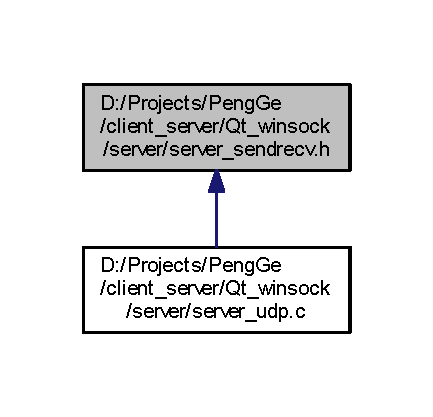
\includegraphics[width=208pt]{server__sendrecv_8h__dep__incl}
\end{center}
\end{figure}
\subsection*{Functions}
\begin{DoxyCompactItemize}
\item 
\hypertarget{server__sendrecv_8h_ae9c6f3f6b0cf2ce3fb01303f983fc97b}{}ssize\+\_\+t {\bfseries server\+\_\+recv} (int fd, void $\ast$inbuf, size\+\_\+t inbytes, struct \hyperlink{structhdr}{hdr} $\ast$hdrdata, struct sockaddr $\ast$cli\+\_\+addr, int $\ast$cli\+\_\+addrlen)\label{server__sendrecv_8h_ae9c6f3f6b0cf2ce3fb01303f983fc97b}

\item 
\hypertarget{server__sendrecv_8h_a68a023db7d8de66e4564760486ebd0d1}{}ssize\+\_\+t {\bfseries server\+\_\+send} (int fd, const void $\ast$outbuf, size\+\_\+t outbytes, const struct \hyperlink{structhdr}{hdr} $\ast$hdrdata, const struct sockaddr $\ast$cli\+\_\+addr, int cli\+\_\+addrlen)\label{server__sendrecv_8h_a68a023db7d8de66e4564760486ebd0d1}

\end{DoxyCompactItemize}


\subsection{Detailed Description}
\begin{DoxyAuthor}{Author}
cxl 
\end{DoxyAuthor}
\begin{DoxyVersion}{Version}
0.\+1 
\end{DoxyVersion}
\begin{DoxyDate}{Date}
2015-\/10-\/10 
\end{DoxyDate}

\hypertarget{server__udp_8c}{}\section{D\+:/\+Projects/\+Peng\+Ge/client\+\_\+server/\+Qt\+\_\+winsock/server/server\+\_\+udp.c File Reference}
\label{server__udp_8c}\index{D\+:/\+Projects/\+Peng\+Ge/client\+\_\+server/\+Qt\+\_\+winsock/server/server\+\_\+udp.\+c@{D\+:/\+Projects/\+Peng\+Ge/client\+\_\+server/\+Qt\+\_\+winsock/server/server\+\_\+udp.\+c}}


The functions prefexed with \char`\"{}s\+\_\+\char`\"{} are static functions.  


{\ttfamily \#include \char`\"{}server\+\_\+udp.\+h\char`\"{}}\\*
{\ttfamily \#include $<$stdlib.\+h$>$}\\*
{\ttfamily \#include $<$stdio.\+h$>$}\\*
{\ttfamily \#include $<$stdint.\+h$>$}\\*
{\ttfamily \#include \char`\"{}udp\+\_\+utility.\+h\char`\"{}}\\*
{\ttfamily \#include \char`\"{}udp\+\_\+types.\+h\char`\"{}}\\*
{\ttfamily \#include \char`\"{}server\+\_\+sendrecv.\+h\char`\"{}}\\*
Include dependency graph for server\+\_\+udp.\+c\+:
\nopagebreak
\begin{figure}[H]
\begin{center}
\leavevmode
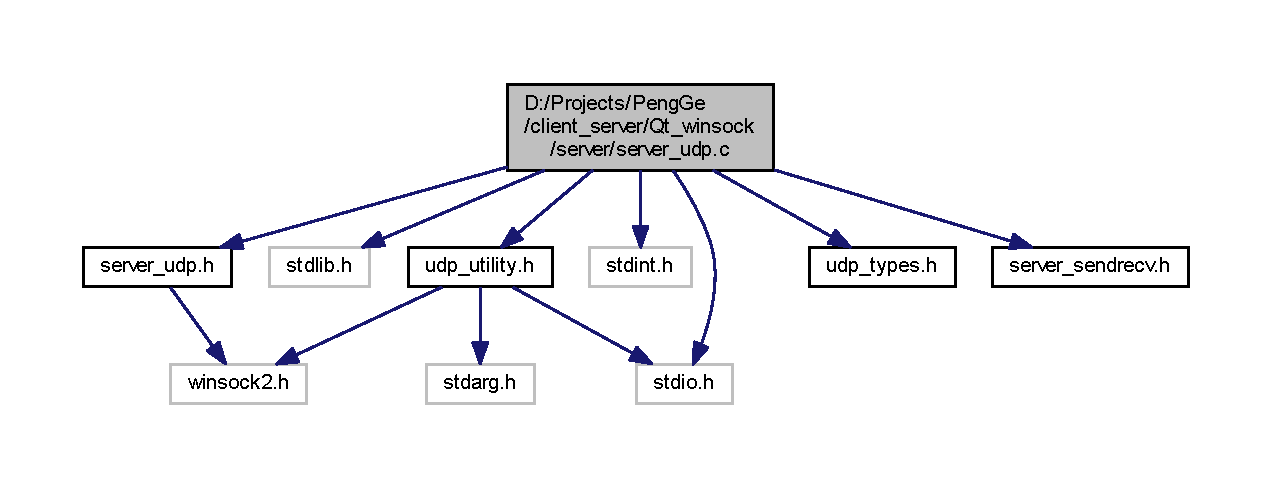
\includegraphics[width=350pt]{server__udp_8c__incl}
\end{center}
\end{figure}
\subsection*{Functions}
\begin{DoxyCompactItemize}
\item 
void \hyperlink{server__udp_8c_a3c6f803a771083053dac5e68b0f6d344}{check\+\_\+args} (int argc, char $\ast$argv\mbox{[}$\,$\mbox{]})
\begin{DoxyCompactList}\small\item\em check\+\_\+args checks whether the arguments are correct. If invalid paramters are passed, this function will give some prompts. \end{DoxyCompactList}\item 
\hypertarget{server__udp_8c_a40ad06b0658b7105ab6de2a697e146a6}{}void {\bfseries init\+\_\+server\+\_\+udp} (struct \hyperlink{structserver__udp}{server\+\_\+udp} $\ast$serv\+\_\+udp)\label{server__udp_8c_a40ad06b0658b7105ab6de2a697e146a6}

\end{DoxyCompactItemize}
\subsection*{Variables}
\begin{DoxyCompactItemize}
\item 
\hypertarget{server__udp_8c_a4520db064bea79e42630a63a529a450c}{}const char $\ast$ {\bfseries g\+\_\+loginmsg\+\_\+header}\label{server__udp_8c_a4520db064bea79e42630a63a529a450c}

\item 
\hypertarget{server__udp_8c_a60cacc9239d0662a686899339cf5b127}{}const char $\ast$ {\bfseries g\+\_\+loginmsg\+\_\+\+S\+U\+C\+C\+E\+S\+S}\label{server__udp_8c_a60cacc9239d0662a686899339cf5b127}

\item 
\hypertarget{server__udp_8c_ab241e51fd6b4014566bd16db0e23de58}{}const char $\ast$ {\bfseries g\+\_\+loginmsg\+\_\+\+F\+A\+I\+L}\label{server__udp_8c_ab241e51fd6b4014566bd16db0e23de58}

\item 
\hypertarget{server__udp_8c_a533bdde78cc9c28ca1a7c9418177f6a7}{}const char {\bfseries g\+\_\+login\+\_\+delimiter}\label{server__udp_8c_a533bdde78cc9c28ca1a7c9418177f6a7}

\end{DoxyCompactItemize}


\subsection{Detailed Description}
The functions prefexed with \char`\"{}s\+\_\+\char`\"{} are static functions. 

\begin{DoxyAuthor}{Author}
cxl 
\end{DoxyAuthor}
\begin{DoxyVersion}{Version}
0.\+1 
\end{DoxyVersion}
\begin{DoxyDate}{Date}
2015-\/09-\/28 
\end{DoxyDate}


\subsection{Function Documentation}
\hypertarget{server__udp_8c_a3c6f803a771083053dac5e68b0f6d344}{}\index{server\+\_\+udp.\+c@{server\+\_\+udp.\+c}!check\+\_\+args@{check\+\_\+args}}
\index{check\+\_\+args@{check\+\_\+args}!server\+\_\+udp.\+c@{server\+\_\+udp.\+c}}
\subsubsection[{check\+\_\+args(int argc, char $\ast$argv[])}]{\setlength{\rightskip}{0pt plus 5cm}void check\+\_\+args (
\begin{DoxyParamCaption}
\item[{int}]{argc, }
\item[{char $\ast$}]{argv\mbox{[}$\,$\mbox{]}}
\end{DoxyParamCaption}
)}\label{server__udp_8c_a3c6f803a771083053dac5e68b0f6d344}


check\+\_\+args checks whether the arguments are correct. If invalid paramters are passed, this function will give some prompts. 

check\+\_\+args simply check whether the program arguments are valid. If the arguments meet the requirements, test\+\_\+args set the port value, else call exit(1).


\begin{DoxyParams}{Parameters}
{\em argc} & \\
\hline
{\em argv\mbox{[}$\,$\mbox{]}} & \\
\hline
\end{DoxyParams}

%--- End generated contents ---

% Index
\backmatter
\newpage
\phantomsection
\clearemptydoublepage
\addcontentsline{toc}{chapter}{Index}
\printindex

\end{document}
